In order to resolve the shortcomings of existing API governance models in the cloud, we propose EAGER, a new model and an architecture
that can be built into the cloud fabrics for providing API governance as a cloud-native feature. We reuse and build upon existing governance
techniques and best practices that have served the SOA community well over the last decade. In this section, we overview the high-level
design of EAGER and provide details on its main components and the policy language.

\subsection{System Design}
EAGER is designed as an extension to existing cloud platforms, especially PaaS offerings. It intercepts all events related to deploying applications
and enforces deployment time governance checks on them. This includes API metadata validation, dependency validation, policy validation and 
API backward compatibility
checking. If either of these checks fails, EAGER halts the deployment of the application and returns an error to the user that initiated the deployment.
In this work we only present the deployment time governance check capabilities of EAGER. However, in this work we also lay the foundation for
providing enforced runtime governance for APIs. We will describe some of these features in this paper, but the final design and implementation of
runtime API governance capability is left as future work.

\begin{figure}
\centering
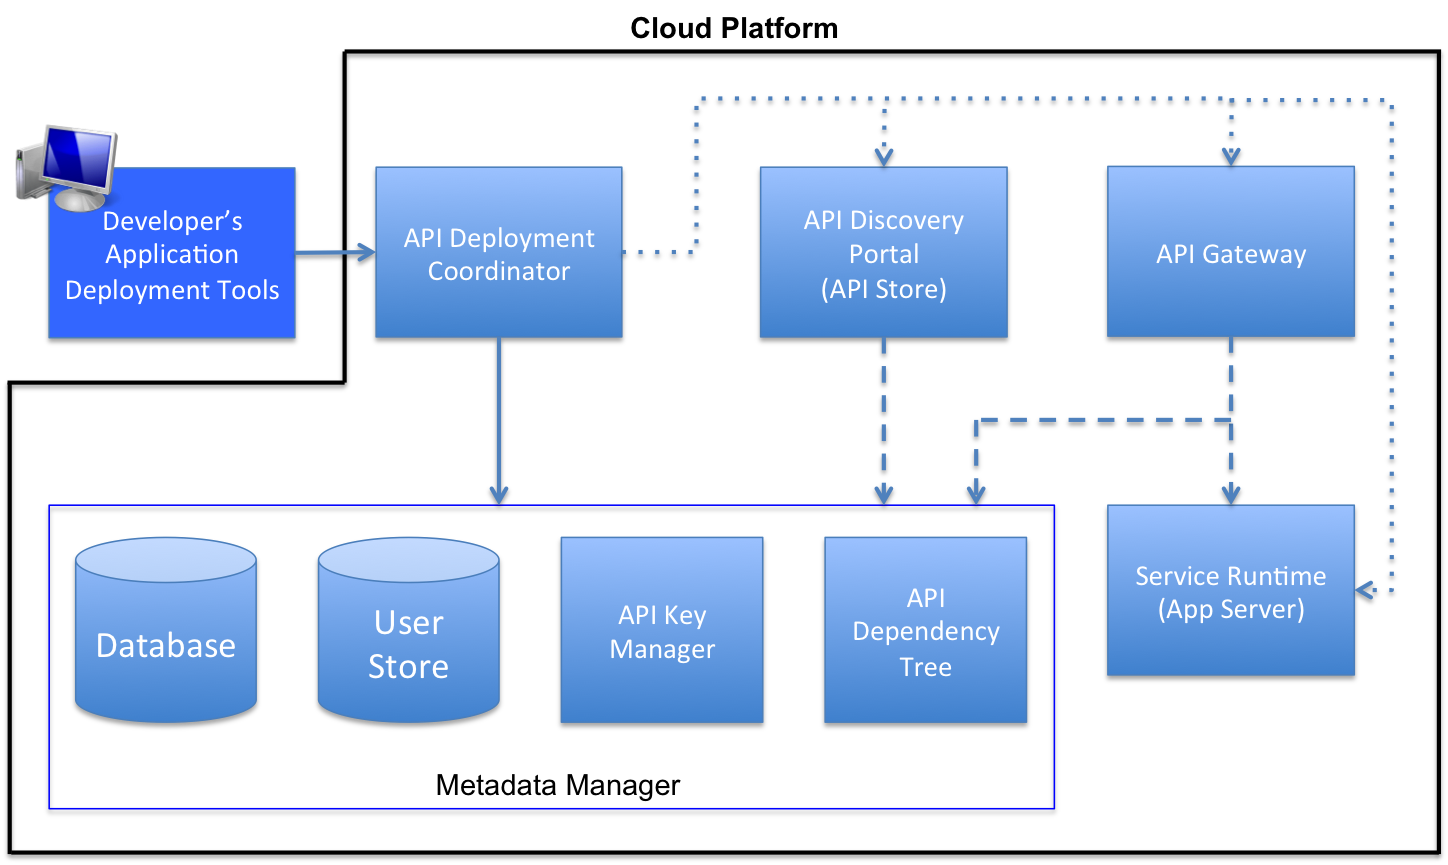
\includegraphics[scale=0.35]{eager_design}
\caption{EAGER Architecture}
\label{fig:eager_design}
\end{figure}

Figure~\ref{fig:eager_design} illustrates the main components of EAGER and their interactions. Solid arrows represent the interactions that take
place during application deployment time, before an application has been checked and validated for deployment. Short-dashed arrows indicate
the interactions that take place during deployment time, after an application has been successfully validated. Long-dashed arrows indicate
interactions during runtime.

EAGER is invoked whenever a developer attempts to deploy a new application, or a new version of an existing application, using the developer
tools available on his/her workstation. In some cloud implementations these tools could be available as an online service accessed by the 
developers via a web browser. In either case, the application deployment request is intercepted by the API Deployment Coordinator in the cloud, which
then queries the Metadata Manager to perform the required governance checks. If a governance check fails, the Deployment Coordinator
will preempt the application deployment and return an error. Otherwise it proceeds to publish the application and the enclosed APIs to an
API Discovery Portal, an API Gateway and also the actual service runtime (typically an application server) that is responsible for hosting
the application in the cloud. 

Note that the proposed architecture does not require major changes to the existing core components of the cloud. All the 
significant components of EAGER that reside in the cloud can be easily implemented as feature additions, on top of what is already available 
in the cloud platform.
The only noteworthy change that is required is the mechanism to intercept application deployment requests and act upon them, before
proceeding to deploy the application to its target runtime. This can be done without having to make any changes to the existing key 
components of the cloud such as application hosting, monitoring, and load balancing.

Following subsections further describe the design and responsibilities of EAGER components.

\subsubsection{API Deployment Coordinator}
API Deployment Coordinator intercepts all application deployment requests and determines whether they are suitable for deployment, based
on a set of policies specified by the cloud or organizational administrators. It receives application deployment requests via a web service interface.
Other components in the cloud and the developer's cloud management tools can use this service interface to remotely submit new applications for
deployment in the cloud. 

An application deployment request contains the name of the application, its version, names and versions of the APIs
exported by the application, detailed API specifications and other API dependencies as declared by the developer. As far as application developers are
concerned, the only things they should explicitly specify are the name and version of the application and the list of dependencies (i.e. APIs consumed
by the application). All other metadata can be computed automatically either at the client side or at the server side by performing introspection on the
application source code. In our prototype implementation of EAGER, we have developed special tools that developers can integrate into their
development environment that performs these metadata calculations, including the automatic generation of API specifications, at the build-time
of an application.

The API specifications used to describe the web APIs should describe the operations and the form (schema) of their inputs and outputs with sufficient 
details. Any suitable standard API description language can be used for this purpose, as long as it clearly describes the schema of the requests and
responses, and we use the same language to describe all APIs deployed via EAGER. For describing REST interfaces, we can use Web Application
Description Language (WADL), Swagger, RAML or any other language that provides similar functionality. Our research currently focuses on RESTful 
services only, but our design can also be adapted to govern SOAP services in the cloud, in which case Web Services Description Language 
(WSDL) can be used to create API specifications.

When a new deployment request is received, API Deployment Coordinator inspects the enclosed application metadata to see if it encloses any web
APIs. If the application exports at least one API, it makes a call to the Metadata Manager and pulls all the existing metadata related to that API. If
the Metadata Manager cannot locate any data related to the APIs in question, API Deployment Coordinator assumes those APIs to be brand new
APIs (i.e. no previous versions of those APIs have been deployed in the cloud), and proceeds to the next step of the governance check phase, which is policy
validation. However, if any metadata regarding the APIs are found, then the API Deployment Coordinator is dealing with a potential API update. In this
case, the Deployment Coordinator compares the old API specifications with the latest ones provided in the application deployment request to see if
they are operation and type compatible.

To perform this API compatibility verification, the API Deployment Coordinator checks to see whether the latest specification of an API contains all 
the operations available in the old specification. If the latest API specification is missing at least one operation that it used to have, the Deployment Coordinator
reports this to the user and aborts the deployment, since this may break some applications that already depend on the missing operations. 
If all the past operations are also present in the latest specification, the Deployment Coordinator performs a type check to make sure that 
all past and present operations are type compatible. This is done by performing recursive introspection on the input and output types declared in the
API specifications. However, instead of looking for exact matches, EAGER looks for ``type compatibility'' based on the following rules inspired by Hoare
logic and the rules of type inheritance from object oriented programming world:
\begin{itemize}
\item New version of an input type is compatible with the old version of an input type, if the new version contains either all or less attributes as the 
old version, and any new attributes that are not present in the old version are optional.
\item New version of an output type is compatible with the old version of an output type, if the new version contains either all or more attributes as the 
old version.
\end{itemize}
In addition to the type checks, API Deployment Coordinator may also look for the compatibility among other parameters declared in the API specifications
such as HTTP methods, mime types and URL patterns.


\subsubsection{Metadata Manager}
\subsubsection{API Discovery Portal}
\subsubsection{API Gateway}